\section{Research Design}
\label{sec:research-design}

This section defines the research objective, research questions, research method, produced artifacts, data and materials, coverage definition, evaluation plan, and scope of the study.

\subsection{Research objective}
\label{subsec:research-objective}

Stakeholders such as product owners typically work from a requirements view of the system, for example through user stories, whereas scriptless GUI testing tools produce an execution view in the form of low-level execution evidence, such as visited GUI states and performed actions. This disconnect makes it difficult to answer a basic assurance question: \emph{which user stories have actually been exercised by testing?}

The objective of this research is to develop and evaluate a method that establishes \emph{requirements traceability} from user stories to execution evidence in GUI State Models, thereby enabling \emph{requirements coverage} reporting for scriptless GUI testing. The method will be developed and evaluated using TESTAR-generated GUI State Models, represented as states, actions, and transitions and exported to JSON for analysis. It will trace the essential steps or acceptance criteria of a user story to corresponding execution evidence in a given GUI State Model and report coverage per user story as \emph{not covered}, \emph{partially covered}, or \emph{fully covered}. The assessment is explicitly bounded by the execution evidence captured in the available GUI State Model.

\subsection{Research questions}
\label{subsec:research-questions}

\paragraph{Main research question (MRQ).}
\begin{quote}
How can user stories be traced to execution evidence in GUI State Models to assess requirements coverage in scriptless GUI testing?
\end{quote}

\paragraph{Sub-questions.}
\begin{description}
    \item[RQ1:] What information and representation are needed from user stories and GUI State Models to establish meaningful trace links?
    \item[RQ2:] How accurate and practically useful is the proposed method in a case study using TESTAR-generated GUI State Models?
\end{description}

\subsection{Research method}
\label{subsec:research-method}

This study follows a \emph{design science} approach in which an artifact is designed, implemented, and evaluated in context. The primary artifact is a traceability method, supported by a prototype, that links user stories to execution evidence in GUI State Models and produces story-level requirements coverage assessments.

The design activities are iterative. Candidate linking strategies will be implemented, applied to real artifacts, and refined based on observed performance, qualitative inspection, and error analysis. The resulting method will be evaluated through a case study on a selected System Under Test (SUT) using TESTAR-generated GUI State Models.

\subsection{Research method}
\label{subsec:research-method}

This study follows a \emph{design science} approach~\citep{peffers2007design} in which an artifact is designed, implemented, and evaluated in context. The primary artifact is a traceability method, supported by a prototype, that links user stories to execution evidence in GUI State Models and produces story-level requirements coverage labels.

The design activities are iterative. Candidate linking strategies will be implemented, applied to real artifacts, and refined based on observed performance, qualitative inspection, and error analysis. The resulting method will be evaluated through a case study on a selected System Under Test (SUT) using TESTAR-generated GUI State Models.

\subsection{Research method}
\label{subsec:research-method}

This study follows a \emph{design science} approach~\citep{peffers2007design} in which an artifact is designed, implemented, and evaluated in context. The primary artifact is a traceability method, supported by linking rules, a coverage assessment procedure, and a prototype implementation, that links user stories to execution evidence in GUI State Models and produces story-level requirements coverage assessments for scriptless GUI testing.

The design activities are iterative. Candidate linking strategies will be implemented, applied to development artifacts, and refined based on observed performance, qualitative inspection, and error analysis. The resulting method will then be subjected to empirical evaluation using separate evaluation artifacts derived from TESTAR-generated GUI State Models.

The empirical component of the study is an \emph{evaluation in context}. The method will be applied in the context of a selected System Under Test (SUT) to assess whether it can establish meaningful trace links between user stories and execution evidence and whether the resulting coverage assessments are accurate and practically useful. Where relevant, results may also be compared across different runs or settings to assess robustness.



This research follows a \emph{Design Science Research} (DSR) approach, because its primary goal is to design and evaluate an artifact that addresses a practical problem in software testing. To structure the study, the research uses the \emph{Design Science Research Methodology} (DSRM) of \citet{peffers2007design}, which organizes the work into problem identification, objective definition, design and development, demonstration, evaluation, and communication.

The primary artifact is a traceability method that links user stories to execution evidence in GUI State Models and supports requirements coverage assessment for scriptless GUI testing. This method is operationalized through supporting artifacts, namely a traceability model and linking rules, a coverage assessment procedure, and a prototype implementation.

Methodologically, the study is primarily \emph{applied} rather than fundamental, because it aims to solve a practical traceability problem in a specific software-testing context. It is also \emph{exploratory and evaluative}: exploratory because the most suitable way to represent and link user stories to GUI State Model evidence is not known in advance, and evaluative because the resulting artifact must be assessed for accuracy and practical usefulness. In terms of reasoning, the study is primarily \emph{abductive and iterative} rather than purely inductive or deductive, since candidate solutions will be designed, confronted with empirical artifacts, and refined based on observed mismatches and performance.

The empirical component of the research uses \emph{mixed methods}. Quantitative analysis will be used to evaluate trace link quality and story-level coverage outcomes, while qualitative analysis will be used for structured inspection, interpretation of ambiguous cases, and error analysis. The study relies mainly on \emph{primary data and materials}, namely user stories, TESTAR-generated GUI State Models, logs, and a manually constructed reference set. Sampling is \emph{purposive} rather than random, because the selected SUT, user stories, and reference subset will be chosen for their relevance to the research objective. The evaluation is expected to be predominantly \emph{cross-sectional}, focusing on selected versions and generated models rather than long-term evolution over time. Because the artifact is evaluated using selected software systems and controlled testing configurations, the study is closer to \emph{controlled empirical evaluation} than to field research. The design phase is relatively \emph{flexible}, whereas the final evaluation will follow a more \emph{fixed} procedure to support consistent interpretation of results.

The design activities are iterative. Candidate linking strategies will be implemented, applied to development artifacts, and refined based on observed performance, qualitative inspection, and error analysis. The resulting method will then be evaluated on separate evaluation artifacts derived from TESTAR-generated GUI State Models.



\subsubsection{Produced artifacts}
\label{subsubsec:produced-artifacts}

The research will produce the following artifacts:

\begin{description}
    \item[A1 --- Traceability model and linking rules:]
    A defined representation of trace links between user stories and GUI State Model evidence, including states, actions, and transitions. Where applicable, the model will also define link semantics and confidence scoring.

    \item[A2 --- Coverage assessment procedure:]
    A procedure that maps the evidence linked to a user story to a coverage assessment, expressed at minimum through the labels \emph{not covered}, \emph{partially covered}, and \emph{fully covered}, using explicit decision rules.

    \item[A3 --- Prototype implementation:]
    A prototype that ingests user stories and TESTAR-generated GUI State Models, generates candidate trace links, supports review or confirmation where needed, and produces requirements coverage reports.
\end{description}

\subsubsection{Data and materials}
\label{subsubsec:data-materials}

The study uses the following data and materials:

\begin{description}
    \item[D1 --- System Under Test (SUT) and configuration:]
    A selected SUT version and its documented runtime and test configuration, including environment, preconditions, and test data, to support reproducibility.

    \item[D2 --- User stories:]
    A set of functional requirements expressed as user stories for the SUT. Each story will have a stable identifier.

    \item[D3 --- GUI State Models:]
    Development and evaluation GUI State Models generated for the SUT using TESTAR. These contain states, actions, transitions, and relevant logging metadata and serve as the primary source of execution evidence.

    \item[D4 --- TESTAR configuration and logs:]
    The TESTAR version, the relevant exploration and logging settings used to generate D3, and the logs needed to interpret model elements.

    \item[D5 --- Reference set (ground truth subset):]
    A manually constructed reference set for a representative subset of user stories and model evidence. It includes expected trace links, where feasible, and story-level coverage labels.
\end{description}






\subsection{Evaluation and validation}
\label{subsec:evaluation-validation}

The evaluation assesses whether the proposed method answers the research questions by measuring the quality of produced trace links and story-level coverage labels on TESTAR-generated GUI State Models.

\subsubsection{Study design}

A case study will be performed on the selected SUT (D1) using user stories (D2) and one or more generated GUI State Models (D3). Where multiple models are available, for example from different runs or exploration settings, the study will compare results across models to assess robustness.

\subsubsection{Measures}

Two types of outcomes will be evaluated:

\begin{itemize}
    \item \textbf{Trace link quality:}
    where D5 contains link-level labels, precision, recall, and F1 will be reported for the produced trace links.

    \item \textbf{Coverage label quality:}
    agreement between predicted and reference story-level coverage labels in D5 will be reported using accuracy and macro-F1.
\end{itemize}

In addition, the evaluation will include an \textbf{error analysis} describing common failure modes, such as ambiguous UI labels, missing exploration paths, or mismatched terminology between user stories and GUI evidence.

\subsubsection{Ground truth strategy}

The reference set (D5) will be created through structured manual inspection of the GUI State Models and supporting artifacts. Labeling rules and assumptions will be documented. If feasible, a second reviewer will label a subset of the data to assess consistency. Otherwise, uncertainties and disagreements will be recorded and resolved through explicit adjudication.

\begin{table}[h!tb]
    \centering
    \caption{Evaluation mapping from research questions to outputs, data, and validation approach.}
    \label{tab:rq-validation-mapping}
    \begin{tabular}{p{1.6cm}p{4.0cm}p{4.2cm}p{5.0cm}}
        \toprule
        \textbf{RQ} & \textbf{Primary outputs} & \textbf{Required data} & \textbf{Validation approach} \\
        \midrule
        MRQ & A1--A3 & D2--D4 & End-to-end demonstration producing trace links and story-level coverage labels. \\
        RQ1 & A1, A2 & D2, D3 & Verify that the chosen representations enable consistent linking and explicit coverage decisions; spot-check on a representative subset. \\
        RQ2 & A1--A3 & D3, D5 & Quantitative evaluation of trace links and coverage labels, complemented by error analysis; compare across runs where available. \\
        \bottomrule
    \end{tabular}
\end{table}

\subsection{Scope and limitations}
\label{subsec:scope-limitations}

This research focuses on \textbf{functional requirements} that can be assessed through GUI interactions and observable UI outcomes. The results are inherently bounded by the exploration coverage captured in the available GUI State Model evidence. Accordingly, a label of \emph{not covered} means \emph{not covered in the available model evidence}, not necessarily absent from the system.




% \section{Research Design}
% \label{sec:research-design}

% This section defines the research objective, research questions, research method, produced artifacts, data and materials, and the evaluation plan.

% % \section{Research}
% % \label{sec:research}

% % This section presents the research objective, research questions, and research method, including the artifacts, data and materials, and validation.

% \subsection{Research objective}
% \label{subsec:research-objective}

% In practice, stakeholders such as product owners manage and report progress at the level of requirements (e.g., user stories),
% while scriptless GUI testing tools primarily produce low-level execution evidence (e.g., visited GUI states and performed actions).
% This disconnect makes it difficult to answer a basic assurance question: \emph{which user stories have actually been exercised by testing?}

% The objective of this research is to develop and evaluate a method that establishes requirements traceability from user stories
% to test execution evidence in GUI State Models, enabling \emph{requirements coverage} reporting for scriptless GUI testing.
% The method is developed and evaluated using TESTAR-generated GUI State Models (states, actions, and transitions) exported to JSON.
% Coverage is reported per user story as \emph{not covered}, \emph{partially covered}, or \emph{fully covered}, where the assessment is
% bounded by the execution evidence captured in the available model(s).

% \subsection{Research objective}
% \label{subsec:research-objective}

% Scriptless GUI testing tools can generate large amounts of low-level execution evidence (e.g., actions and visited GUI states),
% while product and project stakeholders typically reason about progress and quality at the level of requirements (e.g., user stories).
% The objective of this research is to develop and evaluate a method that connects these two views by establishing
% \emph{requirements traceability} from user stories to test execution evidence in GUI State Models.

% Concretely, the method will trace user stories to evidence in a TESTAR-generated GUI State Model (states, actions, and transitions)
% and will compute \emph{requirements coverage} per user story using three categories:
% \emph{not covered}, \emph{partially covered}, and \emph{fully covered}, where coverage is defined with respect to the available
% execution evidence captured in the model (i.e., bounded by exploration).

% % \subsection{Research Objective}
% % \label{subsec:research-objective}

% % The objective of this research is to bridge the gap between requirements-oriented software development and execution-oriented scriptless testing by improving \emph{requirements traceability}. Concretely, this research develops and evaluates a method that traces functional requirements expressed as user stories to test execution evidence in GUI State Models (states, actions, and transitions). The method is applied to TESTAR-generated GUI State Models and assesses \emph{execution completeness} for each user story (not covered, partially covered, or fully covered). The resulting traceability information enables requirements-oriented reporting and evaluation through metrics such as \emph{requirements coverage}.

% \subsection{Research questions}
% \label{subsec:research-questions}

% \paragraph{Main research question (MRQ).}
% \begin{quote}
% How can user stories be traced to test execution evidence in GUI State Models to assess requirements coverage in scriptless GUI testing?
% \end{quote}

% \paragraph{Sub-questions.}
% \begin{description}
%     \item[RQ1:] What information and representation are needed from user stories and GUI State Models to establish meaningful trace links?
%     \item[RQ2:] How accurate and practically useful is the proposed method in a case study using TESTAR-generated GUI State Models?
% \end{description}

% % \subsection{Research Questions}
% % \label{subsec:research-questions}

% % The research objective is addressed through the following main research question:

% % \begin{description}
% %     \item[MRQ:]
% %     How can user stories be traced to test execution evidence in GUI State Models to assess user story execution completeness in scriptless GUI testing?
% % \end{description}

% % This main research question is refined into the following sub-questions:

% % \begin{description}
% %     \item[RQ1:]
% %     How can user stories be transformed into a structured representation suitable for matching against GUI State Models?

% %     \item[RQ2:]
% %     How can user story steps be traced to test execution evidence in GUI State Models?

% %     \item[RQ3:]
% %     How can user story execution completeness (not covered, partially covered, or fully covered) be assessed from traced test execution evidence in GUI State Models?

% %     \item[RQ4:]
% %     How effective is the proposed method when applied to TESTAR-generated GUI State Models?
% % \end{description}

% \subsection{Research method}
% \label{subsec:research-method}

% This study follows a \emph{design science} approach: it designs an artifact (a traceability method, implemented as a prototype)
% and evaluates it in context through a case study. The design activities are iterative: candidate linking strategies are implemented,
% observed on real artifacts, and refined based on measured performance and error analysis.

% % \subsection{Research Method}
% % \label{subsec:research-method}

% % This research follows the \emph{Design Science Research Methodology (DSRM)} proposed by \citet{peffers2007design}. DSRM is appropriate because the primary contribution is an artifact: a traceability method, implemented as a prototype, that links functional requirements expressed as user stories to test execution evidence in GUI State Models. The method consists of several components (A1--A4) that are designed and refined iteratively.

% % In terms of research type, this study is \emph{design science research} with an \emph{empirical evaluation} in the form of a \emph{case study} on a selected System Under Test (SUT) using TESTAR-generated GUI State Models. The design phase includes an \emph{exploratory} element, as multiple tracing strategies can be investigated before selecting and evaluating the most suitable approach.

% % \begin{figure}[h!tb]
% %     \centering
% %     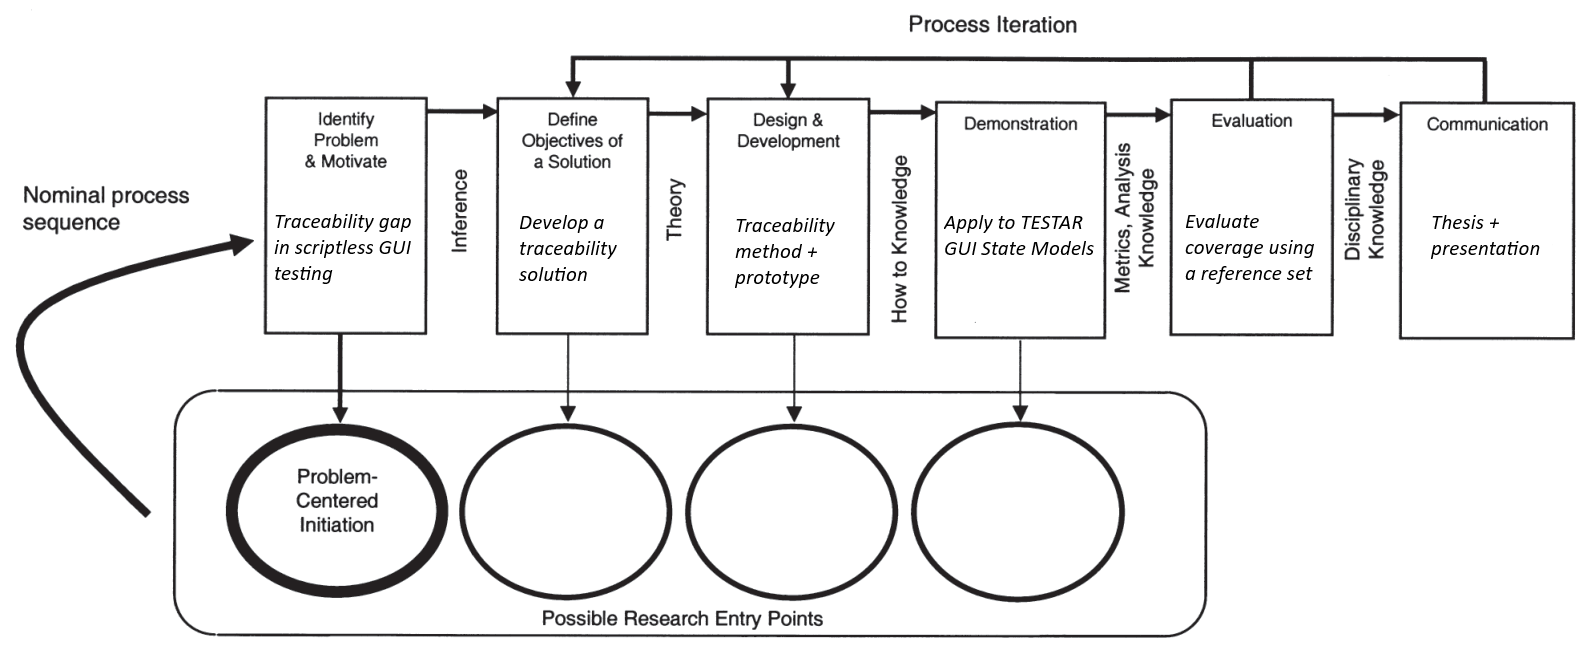
\includegraphics[width=0.95\textwidth]{dsrm-process-model}
% %     \caption{Adapted DSRM process model based on \citet{peffers2007design}.}
% %     \label{fig:dsrm-process-model}
% % \end{figure}

% % Figure~\ref{fig:dsrm-process-model} summarizes the adapted DSRM process model used to structure the research activities. The activities below list the main inputs and outputs. Identifiers refer to method components (A1--A4) and data and materials (D1--D5) defined later in this section.

% % \begin{description}
% %     \item[DSRM-A1 --- Problem identification and motivation:]
% %     Identify the traceability gap between user stories and test execution evidence in GUI State Models, and derive requirements for a solution. \\
% %     \textbf{Inputs:} user stories (D2), GUI State Models (D3). \\
% %     \textbf{Outputs:} problem statement, scope, solution requirements.

% %     \item[DSRM-A2 --- Define objectives of a solution:]
% %     Define design objectives and success criteria for story formalization, tracing, completeness assessment, and reporting. \\
% %     \textbf{Inputs:} outputs of DSRM-A1. \\
% %     \textbf{Outputs:} design objectives, evaluation criteria.

% %     \item[DSRM-A3 --- Design and development:]
% %     Design and implement the method and prototype, producing the main method components. \\
% %     \textbf{Inputs:} SUT configuration (D1), user stories (D2), GUI State Models (D3), scriptless GUI testing tool configuration (D4). \\
% %     \textbf{Outputs:} user story formalization (A1), tracing method (A2), completeness assessment (A3), prototype implementation (A4).

% %     \item[DSRM-A4 --- Demonstration:]
% %     Apply the prototype to GUI State Models to produce trace links and completeness outcomes and gather refinement feedback. \\
% %     \textbf{Inputs:} prototype (A4), user stories (D2), GUI State Models (D3). \\
% %     \textbf{Outputs:} traceability outputs, refinement feedback for A1--A4.

% %     \item[DSRM-A5 --- Evaluation:]
% %     Evaluate trace links and completeness outcomes against the reference set and analyze failure modes. \\
% %     \textbf{Inputs:} tracing method (A2), completeness assessment (A3), prototype (A4), GUI State Models (D3), reference set (D5). \\
% %     \textbf{Outputs:} evaluation results, failure-mode analysis.

% %     \item[DSRM-A6 --- Communication:]
% %     Document the method components, evaluation results, limitations, and implications. \\
% %     \textbf{Inputs:} outputs of DSRM-A1--A5. \\
% %     \textbf{Outputs:} thesis and supporting documentation.
% % \end{description}

% \subsubsection{Produced artifacts}
% \label{subsubsec:produced-artifacts}

% The research will produce the following artifacts:

% \begin{description}
%     \item[A1 --- Traceability model and linking rules:]
%     A defined representation of trace links between (i) user stories and (ii) GUI State Model evidence
%     (states, actions, transitions), including link semantics and confidence scoring where applicable.

%     \item[A2 --- Coverage assessment procedure:]
%     A procedure that maps evidence linked to a user story to a coverage label
%     (\emph{not covered}, \emph{partially covered}, \emph{fully covered}), using explicit decision rules.

%     \item[A3 --- Prototype implementation:]
%     A prototype that ingests user stories and TESTAR GUI State Models, generates candidate links, supports review/confirmation
%     (if needed), and produces coverage reports.
% \end{description}

% % \subsubsection{Method components}
% % \label{subsubsec:artifacts}

% % The traceability method consists of these components:

% % \begin{description}
% %     \item[A1 --- User story formalization:]
% %     A structured, machine-readable representation of user stories that makes required steps and expected UI outcomes explicit for analysis and matching.

% %     \item[A2 --- Tracing method:]
% %     A method to trace user story steps to test execution evidence in GUI State Models and to produce step-level trace links.

% %     \item[A3 --- Completeness assessment:]
% %     A method to assess user story execution completeness (not covered, partially covered, or fully covered) by aggregating step-level trace links.

% %     \item[A4 --- Prototype implementation:]
% %     A prototype implementation that applies A1--A3 to GUI State Models generated by TESTAR.
% % \end{description}

% \subsubsection{Data and materials}
% \label{subsubsec:data-materials}

% The study uses the following data and materials:

% \begin{description}
%     \item[D1 --- System Under Test (SUT) and configuration:]
%     A selected SUT version and a documented configuration (environment, preconditions, and test data) to support reproducibility.

%     \item[D2 --- User stories:]
%     A set of functional requirements expressed as user stories for the SUT. Each story will have a stable identifier.

%     \item[D3 --- GUI State Models:]
%     One or more GUI State Models generated for the SUT using TESTAR. These contain states, actions, transitions, and logging metadata
%     and serve as the primary execution evidence source.

%     \item[D4 --- TESTAR configuration and logs:]
%     The TESTAR version and relevant exploration/logging settings used to generate D3, plus logs needed to interpret model elements.

%     \item[D5 --- Reference set (ground truth subset):]
%     A manually constructed reference set for a representative subset of user stories and model evidence. It includes:
%     (i) expected trace links (where feasible) and (ii) story-level coverage labels.
% \end{description}

% % \subsubsection{Data and materials}
% % \label{subsubsec:data-materials}

% % The research uses these data and materials:

% % \begin{description}
% %     \item[D1 --- System Under Test (SUT) and configuration:]
% %     A selected SUT version and a documented test configuration (e.g., environment settings, test data accounts, and relevant preconditions) to support reproducible testing and model generation.

% %     \item[D2 --- User stories:]
% %     A set of functional requirements expressed as user stories for the selected SUT.

% %     \item[D3 --- GUI State Models:]
% %     One or more GUI State Models generated for the selected SUT using a scriptless GUI testing tool (TESTAR in this research). These models contain states, actions, and transitions and constitute the primary source of test execution evidence used for tracing and completeness assessment.

% %     \item[D4 --- Scriptless GUI testing tool and configuration:]
% %     The scriptless GUI testing tool used in this study, including the TESTAR version and the relevant exploration and logging settings.

% %     \item[D5 --- Reference set for evaluation:]
% %     A manually constructed reference set for a representative subset of stories and executions, including story-level completeness labels and, where applicable, step-level trace links.
% % \end{description}

% \subsection{Coverage definition}
% \label{subsec:coverage-definition}

% Coverage is defined \emph{with respect to the available GUI State Model evidence}.

% \begin{description}
%     \item[Not covered:] No convincing evidence in the GUI State Model can be traced to the user story.
%     \item[Partially covered:] Some evidence supports parts of the user story, but at least one essential element is missing.
%     \item[Fully covered:] The GUI State Model contains sufficient evidence to support all essential elements of the user story.
% \end{description}

% The method will operationalize ``essential elements'' using the chosen story representation (RQ1), for example:
% key user actions, required navigation, and required observable outcomes.

% \subsection{Evaluation and validation}
% \label{subsec:evaluation-validation}

% The evaluation assesses whether the method answers the research questions by measuring link quality and coverage classification
% quality on TESTAR-generated GUI State Models.

% \subsubsection{Study design}
% A case study will be performed on the selected SUT (D1), using user stories (D2) and one or more generated GUI State Models (D3).
% Where multiple models are available (e.g., different runs or exploration settings), the study will compare results across models to
% assess robustness.

% \subsubsection{Measures}
% Two types of outcomes will be evaluated:

% \begin{itemize}
%     \item \textbf{Trace link quality (where D5 contains link-level labels):}
%     precision, recall, and F1 for the produced trace links.
%     \item \textbf{Coverage label quality (story-level):}
%     agreement between predicted and reference labels in D5, reported as accuracy and macro-F1 (multi-class).
% \end{itemize}

% In addition, the evaluation will include a short \textbf{error analysis} describing common failure modes
% (e.g., ambiguous UI labels, missing exploration paths, or mismatched terminology).

% \subsubsection{Ground truth strategy}
% The reference set (D5) will be created via structured manual inspection of the GUI State Model and supporting artifacts.
% Labeling rules and assumptions will be documented. If feasible, a second reviewer will label a subset to check consistency;
% otherwise, disagreements and uncertainties will be recorded and resolved through explicit adjudication.

% \begin{table}[h!tb]
%     \centering
%     \caption{Evaluation mapping from research questions to outputs, data, and validation approach.}
%     \label{tab:rq-validation-mapping}
%     \begin{tabular}{p{1.6cm}p{4.0cm}p{4.2cm}p{5.0cm}}
%         \toprule
%         \textbf{RQ} & \textbf{Primary outputs} & \textbf{Required data} & \textbf{Validation approach} \\
%         \midrule
%         MRQ & A1--A3 & D2--D4 & End-to-end demonstration producing trace links and story-level coverage labels. \\
%         RQ1 & A1, A2 & D2, D3 & Verify that the chosen representations enable consistent linking and explicit coverage decisions; spot-check on a representative subset. \\
%         RQ2 & A1--A3 & D3, D5 & Quantitative evaluation (precision/recall/F1 for links where possible; accuracy/macro-F1 for coverage labels) plus error analysis; compare across runs if available. \\
%         \bottomrule
%     \end{tabular}
% \end{table}

% % \subsection{Validation}
% % \label{subsec:validation}

% % Validation assesses whether the proposed method and prototype address the research questions by evaluating their outputs on TESTAR-generated GUI State Models (D3). The evaluation uses a manually constructed reference set (D5) for a representative subset of stories and executions.

% % For tracing (RQ2), produced step-level trace links are compared to the reference set where available, complemented by targeted qualitative inspection of mismatches. For execution completeness (RQ3--RQ4), assessed user stories (not covered, partially covered, or fully covered) are compared to the reference labels in D5 and reported using standard multi-class metrics such as accuracy and macro-F1. In addition, failure-mode analysis is performed to characterize common sources of incorrect trace links or completeness outcomes.

% % The reference set (D5) will be created through manual inspection of the GUI State Models and, where available, supporting execution artifacts. Labeling decisions and assumptions will be documented; disagreements will be resolved through adjudication to make interpretation decisions explicit. When multiple GUI State Models are available (e.g., from different runs or configurations), results will be compared across models to assess robustness and sensitivity to testing settings.

% % Throughout the evaluation, \emph{not covered} is interpreted as \emph{not covered in the available GUI State Model evidence}, acknowledging that exploration coverage may limit what can be concluded from a given model.

% % \begin{table}[h!tb]
% %     \centering
% %     \caption{Validation approach aligned with research questions, method components, and required data.}
% %     \label{tab:validation}
% %     \begin{tabular}{p{1.6cm}p{3.4cm}p{3.6cm}p{6.0cm}}
% %         \toprule
% %         \textbf{RQ} & \textbf{Primary outputs} & \textbf{Required data} & \textbf{Validation approach} \\
% %         \midrule
% %         RQ1 & A1 & D2 & Check that stories can be represented consistently and are suitable for matching/tracing; spot-check on a representative subset. \\
% %         RQ2 & A2, A4 & D2, D3, D4, D5 & Compare produced trace links to the reference set where available; analyze mismatches and failure cases. \\
% %         RQ3 & A3, A4 & D3, D4, D5 & Compare assessed completeness labels to D5 (not covered/partially covered/fully covered); report multi-class metrics and inspect misclassifications. \\
% %         RQ4 & A1--A4 & D3, D5 & Evaluate overall effectiveness on TESTAR-generated models; report performance and failure-mode analysis; assess robustness across runs/configurations when available. \\
% %         \bottomrule
% %     \end{tabular}
% % \end{table}

% \subsection{Scope and limitations}
% \label{subsec:scope-limitations}

% This research targets \textbf{functional} requirements that can be validated through GUI interactions and observable UI outcomes.
% Results are inherently bounded by the exploration coverage captured in the GUI State Model: ``not covered'' means
% \emph{not covered in the available model evidence}, not necessarily absent from the system.

% \section{Research Questions}

% This research is guided by the following questions.

% \subsection{Primary research question}
% \textbf{RQ1:} How can requirements traceability be established and maintained for scriptless GUI tests with
% high accuracy and low ongoing effort?

% \subsection{Secondary research questions}
% \textbf{RQ2:} Which information sources from scriptless test artifacts (e.g., step text, selectors, assertions,
% logs) contribute most to generating correct requirement--test links?

% \textbf{RQ3:} How stable are requirement--test links under typical evolution scenarios (requirement changes,
% UI refactoring, and test maintenance)?

% \textbf{RQ4:} What is the cost--benefit profile of the proposed approach compared to a baseline (e.g., no
% traceability, or manual-only traceability) in terms of analyst time, link quality, and maintenance effort?

% \subsection{Working hypotheses}
% \begin{itemize}[leftmargin=*]
%     \item \textbf{H1:} A hybrid approach (automated candidate links + human confirmation) achieves higher
%     precision/recall than manual linking at the same effort level.
%     \item \textbf{H2:} Step descriptions and assertions provide stronger signals for traceability than selectors
%     alone, but selectors improve link robustness when text is sparse.
%     \item \textbf{H3:} Link maintenance can be reduced by modeling trace links at multiple granularities
%     (requirement-to-test and requirement-to-step) and by recording rationale for links.
% \end{itemize}

% \section{Methodology}

% \subsection{Research approach}
% This project follows a design science approach: an artifact (traceability method and prototype) is designed,
% implemented, and evaluated in context. The focus is not only on technical correctness but also on practical
% usability and maintenance outcomes.

% \subsection{Proposed traceability model}
% The proposed model represents trace links between:
% \begin{itemize}[leftmargin=*]
%     \item \textbf{Requirements} (identified by stable IDs and short titles),
%     \item \textbf{Scriptless tests} (test-level entities),
%     \item \textbf{Test steps and assertions} (optional finer-grained entities),
%     \item \textbf{Evidence} (execution logs, screenshots, or outcomes where available).
% \end{itemize}

% Links include attributes for:
% \begin{itemize}[leftmargin=*]
%     \item link type (verifies, partially verifies, supports),
%     \item confidence score (for automatically proposed links),
%     \item rationale (short human explanation for acceptance),
%     \item last-validated timestamp and artifact versions.
% \end{itemize}

% \subsection{Link generation and validation}
% The method will generate candidate links using a combination of signals:
% \begin{enumerate}[leftmargin=*]
%     \item \textbf{Text similarity} between requirement statements and test metadata/step descriptions/assertions;
%     \item \textbf{Action semantics} (e.g., mapping ``create order'' requirements to sequences containing create/save);
%     \item \textbf{UI element semantics} where meaningful names exist (labels, accessibility names, stable IDs);
%     \item \textbf{Execution evidence} such as assertion outcomes that correspond to requirement acceptance criteria.
% \end{enumerate}

% Candidates will be presented for human confirmation. Confirmed links are stored in a traceability matrix and
% can be exported for reporting.

% \subsection{Link maintenance under change}
% To support maintenance, the approach will:
% \begin{itemize}[leftmargin=*]
%     \item detect changes in requirements (modified text, split/merge) and flag affected links;
%     \item detect changes in tests (renamed tests, changed step sequences, updated selectors);
%     \item recommend re-validation when confidence drops (e.g., step drift beyond a threshold);
%     \item keep a small, explicit rationale so that future reviewers can understand why a link exists.
% \end{itemize}

% \subsection{Prototype implementation}
% A lightweight prototype will be built to demonstrate feasibility. It will:
% \begin{itemize}[leftmargin=*]
%     \item ingest requirements (e.g., from a structured document or CSV),
%     \item ingest scriptless test exports (tool-dependent; normalized into a common intermediate format),
%     \item generate candidate links with scores,
%     \item store and export confirmed links (CSV/JSON trace matrix),
%     \item support basic change detection and re-validation prompts.
% \end{itemize}

% Tool-specific details will be treated as adapters so that the core method remains reusable.

% \section{Evaluation Plan}

% \subsection{Study design}
% The evaluation will be conducted as a case study on one or more applications that have:
% \begin{itemize}[leftmargin=*]
%     \item a set of documented functional requirements (with IDs),
%     \item an existing scriptless GUI test suite,
%     \item at least one change cycle (requirements update and/or UI changes) to assess maintenance.
% \end{itemize}

% A baseline will be defined for comparison, such as:
% \begin{itemize}[leftmargin=*]
%     \item no explicit traceability (status quo), and/or
%     \item manual linking without automated candidate generation.
% \end{itemize}

% \subsection{Measurements}
% Primary quality measures:
% \begin{itemize}[leftmargin=*]
%     \item \textbf{Precision:} proportion of proposed/confirmed links that are correct.
%     \item \textbf{Recall:} proportion of true requirement--test links that are captured.
%     \item \textbf{F1 score:} combined view of precision and recall.
% \end{itemize}

% Maintenance measures:
% \begin{itemize}[leftmargin=*]
%     \item \textbf{Link stability:} proportion of links that remain valid after changes.
%     \item \textbf{Re-validation effort:} time to review and update links after changes.
% \end{itemize}

% Engineering practicality measures:
% \begin{itemize}[leftmargin=*]
%     \item \textbf{Initial setup time:} effort to ingest artifacts and create first trace matrix.
%     \item \textbf{User effort:} analyst time for confirmation and rationale writing.
% \end{itemize}

% \subsection{Ground truth strategy}
% Because traceability is partly judgment-based, ground truth will be established via:
% \begin{itemize}[leftmargin=*]
%     \item independent labeling by at least two reviewers when feasible, or
%     \item a structured review with the supervisor/stakeholder to confirm link correctness,
% \end{itemize}
% with disagreements documented and resolved using explicit criteria.

% \subsection{Threats to validity}
% Key threats and mitigations:
% \begin{itemize}[leftmargin=*]
%     \item \textbf{Construct validity:} metrics may not reflect real assurance value; mitigate by also measuring
%     effort and change impact usefulness.
%     \item \textbf{Internal validity:} reviewer bias; mitigate via clear labeling criteria and (if feasible)
%     cross-review.
%     \item \textbf{External validity:} single-case limitation; mitigate by describing the context precisely and,
%     if feasible, adding a second small case.
%     \item \textbf{Conclusion validity:} small sample sizes; mitigate by reporting confidence intervals or
%     sensitivity analyses where appropriate.
% \end{itemize}




\section{Research Design}
\label{sec:research-design}

This section defines the research objective, research questions, research method, produced artifacts, data and materials, coverage definition, evaluation plan, and scope of the study.

\subsection{Research objective}
\label{subsec:research-objective}

Stakeholders such as product owners typically manage and report progress at the level of requirements, for example through user stories, whereas scriptless GUI testing tools primarily produce low-level execution evidence, such as visited GUI states and performed actions. This disconnect makes it difficult to answer a basic assurance question: \emph{which user stories have actually been exercised by testing?}

The objective of this research is to develop and evaluate a method that establishes \emph{requirements traceability} from user stories to execution evidence in GUI State Models, thereby enabling \emph{requirements coverage} reporting for scriptless GUI testing. The method will be developed and evaluated using TESTAR-generated GUI State Models, represented as states, actions, and transitions and exported to JSON for analysis. Coverage will be reported per user story as \emph{not covered}, \emph{partially covered}, or \emph{fully covered}, where the assessment is explicitly bounded by the execution evidence captured in the available model or models.

\subsection{Research questions}
\label{subsec:research-questions}

\paragraph{Main research question (MRQ).}
\begin{quote}
How can user stories be traced to execution evidence in GUI State Models to assess requirements coverage in scriptless GUI testing?
\end{quote}

\paragraph{Sub-questions.}
\begin{description}
    \item[RQ1:] What information and representation are needed from user stories and GUI State Models to establish meaningful trace links?
    \item[RQ2:] How accurate and practically useful is the proposed method in a case study using TESTAR-generated GUI State Models?
\end{description}

\subsection{Research method}
\label{subsec:research-method}

This study follows a \emph{design science} approach~\citep{peffers2007design} in which an artifact is designed, implemented, and evaluated in context. The primary artifact is a traceability method, supported by a prototype, that links user stories to execution evidence in GUI State Models and produces story-level requirements coverage labels.

The design activities are iterative. Candidate linking strategies will be implemented, applied to real artifacts, and refined based on observed performance, qualitative inspection, and error analysis. The resulting method will be evaluated through a case study on a selected System Under Test (SUT) using TESTAR-generated GUI State Models.

\subsubsection{Produced artifacts}
\label{subsubsec:produced-artifacts}

The research will produce the following artifacts:

\begin{description}
    \item[A1 --- Traceability model and linking rules:]
    A defined representation of trace links between user stories and GUI State Model evidence, including states, actions, and transitions. Where applicable, the model will also define link semantics and confidence scoring.

    \item[A2 --- Coverage assessment procedure:]
    A procedure that maps the evidence linked to a user story to a coverage label
    (\emph{not covered}, \emph{partially covered}, or \emph{fully covered}) using explicit decision rules.

    \item[A3 --- Prototype implementation:]
    A prototype that ingests user stories and TESTAR-generated GUI State Models, generates candidate trace links, supports review or confirmation where needed, and produces requirements coverage reports.
\end{description}

\subsubsection{Data and materials}
\label{subsubsec:data-materials}

The study uses the following data and materials:

\begin{description}
    \item[D1 --- System Under Test (SUT) and configuration:]
    A selected SUT version and a documented configuration, including environment, preconditions, and test data, to support reproducibility.

    \item[D2 --- User stories:]
    A set of functional requirements expressed as user stories for the SUT. Each story will have a stable identifier.

    \item[D3 --- GUI State Models:]
    One or more GUI State Models generated for the SUT using TESTAR. These contain states, actions, transitions, and relevant logging metadata and serve as the primary source of execution evidence.

    \item[D4 --- TESTAR configuration and logs:]
    The TESTAR version and the relevant exploration and logging settings used to generate D3, together with logs needed to interpret model elements.

    \item[D5 --- Reference set (ground truth subset):]
    A manually constructed reference set for a representative subset of user stories and model evidence. It includes expected trace links, where feasible, and story-level coverage labels.
\end{description}

\subsection{Coverage definition}
\label{subsec:coverage-definition}

Coverage is defined \emph{with respect to the available GUI State Model evidence}.

\begin{description}
    \item[Not covered:] No convincing execution evidence in the GUI State Model can be traced to the user story.
    \item[Partially covered:] Some execution evidence supports parts of the user story, but at least one essential element is missing.
    \item[Fully covered:] The GUI State Model contains sufficient execution evidence to support all essential elements of the user story.
\end{description}

The method will operationalize ``essential elements'' using the chosen story representation from RQ1, for example through key user actions, required navigation steps, and required observable outcomes.

\subsection{Evaluation and validation}
\label{subsec:evaluation-validation}

The evaluation assesses whether the proposed method answers the research questions by measuring the quality of produced trace links and story-level coverage labels on TESTAR-generated GUI State Models.

\subsubsection{Study design}

A case study will be performed on the selected SUT (D1) using user stories (D2) and one or more generated GUI State Models (D3). Where multiple models are available, for example from different runs or exploration settings, the study will compare results across models to assess robustness.

\subsubsection{Measures}

Two types of outcomes will be evaluated:

\begin{itemize}
    \item \textbf{Trace link quality:}
    where D5 contains link-level labels, precision, recall, and F1 will be reported for the produced trace links.

    \item \textbf{Coverage label quality:}
    agreement between predicted and reference story-level coverage labels in D5 will be reported using accuracy and macro-F1.
\end{itemize}

In addition, the evaluation will include an \textbf{error analysis} describing common failure modes, such as ambiguous UI labels, missing exploration paths, or mismatched terminology between user stories and GUI evidence.

\subsubsection{Ground truth strategy}

The reference set (D5) will be created through structured manual inspection of the GUI State Models and supporting artifacts. Labeling rules and assumptions will be documented. If feasible, a second reviewer will label a subset of the data to assess consistency. Otherwise, uncertainties and disagreements will be recorded and resolved through explicit adjudication.

\begin{table}[h!tb]
    \centering
    \caption{Evaluation mapping from research questions to outputs, data, and validation approach.}
    \label{tab:rq-validation-mapping}
    \begin{tabular}{p{1.6cm}p{4.0cm}p{4.2cm}p{5.0cm}}
        \toprule
        \textbf{RQ} & \textbf{Primary outputs} & \textbf{Required data} & \textbf{Validation approach} \\
        \midrule
        MRQ & A1--A3 & D2--D4 & End-to-end demonstration producing trace links and story-level coverage labels. \\
        RQ1 & A1, A2 & D2, D3 & Verify that the chosen representations enable consistent linking and explicit coverage decisions; spot-check on a representative subset. \\
        RQ2 & A1--A3 & D3, D5 & Quantitative evaluation of trace links and coverage labels, complemented by error analysis; compare across runs where available. \\
        \bottomrule
    \end{tabular}
\end{table}

\subsection{Scope and limitations}
\label{subsec:scope-limitations}

This research focuses on \textbf{functional requirements} that can be assessed through GUI interactions and observable UI outcomes. The results are inherently bounded by the exploration coverage captured in the available GUI State Model evidence. Accordingly, a label of \emph{not covered} means \emph{not covered in the available model evidence}, not necessarily absent from the system.
